\documentclass[crop,border={2pt 2pt 2pt 2pt},tikz]{standalone}
\usepackage{braket}
\usepackage{bbold}
\usepackage{bm}
\usepackage{amsmath}
\usepackage{tikz-3dplot}
% \usepackage{physics}

\usetikzlibrary{backgrounds,decorations.markings, calc}
\tikzset{>=latex}
\tikzset{->-/.style={decoration={
  markings,
  mark=at position .55 with {\arrow{>}}},postaction={decorate}}}
\begin{document}
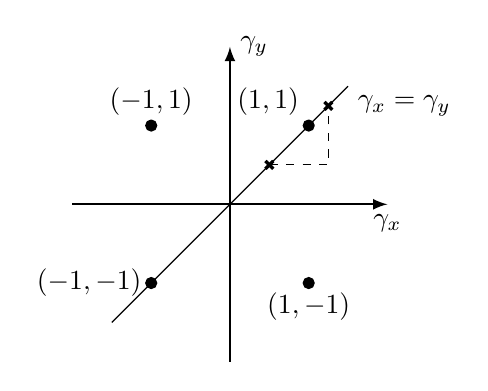
\begin{tikzpicture}[line join = round]
    \draw[black] (-1.5,-1.5) -- (1.5,1.5) node[anchor=north west] {$\gamma_x = \gamma_y$};
    \draw[fill, black] (-1,-1) node[anchor=east] {$(-1,-1)$} circle (2pt) (1,-1) node[anchor=north] {$(1,-1)$} circle (2pt) (-1,1)  node[anchor=south] {$(-1,1)$} circle (2pt) (1,1) node[anchor=south east] {$(1,1)$} circle (2pt);
    \draw[thick,->] (-2,0) -- (2,0) node[anchor=north] {$\gamma_x$};
    \draw[thick,->] (0,-2) -- (0,2) node[anchor=west] {$\gamma_y$};

    \draw[black, very thick] (0.5 -0.05,0.5 -0.05) -- (0.5 + 0.05,0.5+0.05);
    \draw[black, very thick] (0.5 - 0.05,0.5 + 0.05) -- (0.5 + 0.05,0.5 -0.05);

    \draw[black, very thick] (1.25 -0.05,1.25 -0.05) -- (1.25 + 0.05,1.25+0.05);
    \draw[black, very thick] (1.25 - 0.05,1.25 + 0.05) -- (1.25 + 0.05,1.25 -0.05);
    \draw[black, dashed] (0.5,0.5) -- (1.25,0.5) -- (1.25,1.25); 
\end{tikzpicture}
\end{document}